\definecolor{exxetagray}{gray}{0.75}
\definecolor{itemcolor}{RGB}{179,217,255}
\definecolor{usercolor}{RGB}{255,204,179}

\shorthandoff{"}
\chapter{Empfehlungssysteme}
\label{ch:empfehlungssysteme}
% Zeitplan in Readme

\section{Einführung}
\label{ch:empfehlungssysteme:einfuehrung}
Der Begriff des Empfehlungssystems ist im englischsprachigen Raum auch unter Bezeichnungen wie "Recommender System" \cite[S. 1]{lu:2015}, "Recommender Engine" \cite[S. 1]{panigrahi:2016} und "Recommendation System" \cite[S. 1]{ebesu:2018} verbreitet. Er wurde erstmals im Jahr 1997 von \textcite[S. 1]{resnick:1997} geprägt. Dass der Begriff gerade zu diesem Zeitpunkt entstand, ist auf die zur damaligen Zeit stark wachsende Internetnutzung und die damit verbundenen einfachen Möglichkeiten zur Sammlung und Auswertung großer Mengen an Nutzerdaten zurückzuführen \cite[S. xvii]{recommenderSystems:2016}.

Besonders bekannt für den Einsatz von Empfehlungssystemen sind große IT-Konzerne wie Amazon, Facebook, Google und Netflix \cite[S. 1]{zarzour:2018}. Diese Unternehmen nutzen Recommender Engines, um ihren Kunden personalisierte Vorschläge zu den Inhalten ihrer Plattformen anzuzeigen \cite[S. 2]{jeckmans:2013}. Häufig entfällt dabei für den Anwender vollständig die Notwendigkeit einer manuellen Suche \cite[S. 1]{comibingCareer:2013}.

Der Einsatz von Empfehlungssystemen wird in der Literatur kritisch diskutiert. Beispielsweise beobachteten \textcite[S. 17f.]{alfano:2020}, dass das Empfehlungssystem der Videostreaming-Plattform YouTube dazu tendiert, neuen Anwendern zur Verlängerung ihrer Nutzungszeit verschwörungstheoretische Inhalte auszuspielen. Eine Untersuchung von Forschern des sozialen Netzwerks Facebook kam zu dem Ergebnis, dass deren Recommender Engine Nutzern verstärkt Inhalte präsentierte, welche konform mit deren Ideologien waren \cite[S. 2]{bakshy:2015}. \textcite[S. 1ff.]{pariser:2012} prägte für diese Art der Personalisierung den Begriff der Filterblase.

Empfehlungssysteme haben aber auch einen bedeutenden Anteil am wirtschaftlichen Erfolg großer Internetplattformen. So führten beispielsweise \textcite[S. 6f.]{sharma:2015} etwa 30 Prozent des Internetverkehrs beim Online-Händler Amazon unmittelbar auf den Einsatz von Empfehlungssystemen zurück. \textcite[S. 5]{gomezuribe:2016} stellten bei einer Analyse der Streaming-Plattform Netflix fest, dass ca. 80 Prozent der Nutzungszeit auf Videos entfiel, welche Nutzern ohne vorherige Suche von einer Recommender Engine angezeigt wurden.

Um solche Vorschläge generieren zu können, suchen Empfehlungssysteme relevante Inhalte basierend auf den Präferenzen der Anwender aus \cite[S. 1]{das:2017}. Zu diesem Zweck müssen benötigte Nutzerdaten zunächst erhoben und in einer maschinell auswertbaren Struktur gespeichert werden.

\section{Zugrundeliegende Datenstruktur}
\label{ch:empfehlungssysteme:arbeitsweise}
Empfehlungssysteme können die Präferenzen ihrer Nutzer sowohl über explizite als auch implizite Rückmeldungen erfassen. Explizites Feedback erhalten Plattformen beispielsweise über abgegebene Produktbewertungen oder "Gefällt mir"-Angaben in sozialen Netzwerken. Um implizite Rückmeldungen auszuwerten, werden häufig Verhaltensweisen der Nutzer aufgezeichnet. Hierbei kann es sich beispielsweise um Suchverläufe oder die Wiedergabedauer von Videos handeln \cite[S. 3]{pu:2012}.

Das gesammelte Feedback überführen Analysten in die Struktur von Matrizen \cite[S. 11f.]{recommenderSystems:2016}. Ein Beispiel für eine Matrix mit explizit erfassten Bewertungen der Fähigkeiten von Mitarbeitern ist in Tabelle \ref{tbl:empfehlungssysteme:arbeitsweise:tbl1} dargestellt.

\begin{table}[h]
	\centering
	\begin{tabular}{c|c|c|c|c|c|c}
	 & Java & Python & MySQL & MongoDB & HDFS & Spark\\ 
	\hline
	Doe, Jane & ? & 4 & 3 & 3 & ? & ?\\
	Doe, John & 3 & ? & 2 & ? & 1 & ?\\
	Muster, Erika & ? & ? & ? & ? & 5 & 3\\
	Muster, Max & 2 & 3 & 1 & ? & ? & ?
	\end{tabular}
	\caption{Beispiel für die Matrixdarstellung von Fähigkeiten}
	\label{tbl:empfehlungssysteme:arbeitsweise:tbl1}
\end{table}

In Tabelle \ref{tbl:empfehlungssysteme:arbeitsweise:tbl1} sind in der ersten Spalte die Mitarbeiter eines Unternehmens gespeichert. Diese werden als Nutzer (User) bezeichnet. In der Kopfzeile der folgenden Spalten sind verschiedene Fähigkeiten eingetragen. Diese werden Elemente (Items) genannt. In der Mitte der Tabelle befinden sich die Bewertungen (Ratings) der Fähigkeiten jedes Nutzers \cite[S. 1f.]{strub:2016}. Im Beispiel aus Tabelle \ref{tbl:empfehlungssysteme:arbeitsweise:tbl1} wurden die expliziten Beurteilungen auf einer Skala von eins bis fünf vergeben. Diese bewerteten Matrix-Einträge werden  als beobachtet (observed) oder spezifiziert (specified) bezeichnet. Unbewertete Elemente sind mit einem Fragezeichen gekennzeichnet und werden unbeobachtet (unobserved) oder fehlend (missing) genannt \cite[S. 8]{recommenderSystems:2016}.

Zahlreiche Wissenschaftler in der Literatur sind sich einig, dass für die Empfehlung geeigneter Kandidaten für eine Stelle bzw. Projektposition ein einfacher Abgleich zwischen gesuchten und vorhandenen Fähigkeiten in der Matrix eine unzureichende Lösung darstellt \cite[S. 1]{enhancingERecruitment:2012}\cite[S. 1]{faerber:2003}\cite[S. 2]{prospect:2010} und der Komplexität der Aufgabe nicht gerecht wird \cite[S. 1]{malinowski:2008}. So kritisierten beispielsweise \textcite[S. 1f.]{mitre:2014}, dass bei einem solchen Ansatz Synonyme und verwandte Fähigkeit nicht in die Suche einbezogen werden. Um diesem Problem zu begegnen, existieren in der Literatur zahlreiche unterschiedliche Ansätze, Recommender Enginges zu implementieren. Ein verbreitetes Verfahren ist das kollaborative Filtern.
% Einer davon ist die Umsetzung eines wissensbasierten Empfehlungssystems \cite[S. 2f.]{dwivedi:2017}.

\section{Kollaboratives Filtern}
\label{ch:empfehlungssysteme:cf}
Ein Ziel von Verfahren im Bereich des kollaborativen Filterns ist das Vorhersagen unbewerteter Einträge in Tabelle \ref{tbl:empfehlungssysteme:arbeitsweise:tbl1}. Unbeobachtete Werte eines Zielnutzers werden dabei über Ähnlichkeitsberechnungen aus vergebenen Beurteilungen anderer Anwender geschlussfolgert \cite[S. 1]{su:2009}.

\textcite[S. 3]{breese:1998} unterschieden zwischen speicher- (memory-) und modellbasierten (modelbased) Algorithmen. Speicherbasierte Verfahren übertragen sämtliche Nutzer und deren Bewertungen bei der Berechnung von Empfehlungen vollständig in den Hauptspeicher des Rechners. Modellbasierte Verfahren nutzen dagegen Algorithmen aus dem Bereich des Data Minings. Diese werden genutzt, um vor dem Einsatz in der Produktivumgebung statistische Vorhersage-Modelle zu entwickeln \cite[S. 3]{breese:1998}\cite[S. 11]{schafer:2007}. In der Literatur existieren unterschiedliche Ansätze, speicher- und modellbasierte Verfahren zu implementieren.

\subsection{Speicherbasierte Verfahren}
\label{ch:empfehlungssysteme:cf:speicherbasiert}
Um speicherbasierte Verfahren zu entwickeln, werden nachbarschaftsbasierte Algorithmen eingsetzt \cite[S. 29]{recommenderSystems:2016}. Soll hierbei beispielsweise die fehlende Javabewertung von Jane Doe in Tabelle \ref{tbl:empfehlungssysteme:arbeitsweise:tbl1} vorhergesagt werden, erfolgt dies über paarweise Ähnlichkeitsberechnungen \cite[S. 2f.]{bharti:2019}. Verwenden Algorithmen dabei die Ähnlichkeiten zwischen Mitarbeitern bzw. Tabellenzeilen zur Vorhersage, werden diese als nutzerorientiert (user-oriented) bezeichnet. Greifen Verfahren dagegen auf die Gleichartigkeit zwischen Fähigkeiten bzw. Tabellenspalten zurück, werden sie elementorientiert (item-oriented) genannt \cite[S. 1f.]{duong:2018}. Laut \textcite[S. 42]{recommenderSystems:2016} liefern elementorientierte Verfahren häufig präzisere, nutzerorientierte Methoden dafür diversere Ergebnisse. Somit erwartete der Autor, dass die Vorschläge der erstgenannten Ansätze für den Nutzer relevanter erscheinen. Jedoch bemängelte er das hohe Risiko bei elementbasierten Verfahren, dass dem Anwender aufgrund der hohen Ähnlichkeit der Elemente kein einziger Vorschlag gefallen könnte, wenn nur eine Empfehlung unzutreffend ist.

Bei der Implementierung nachbarschaftsbasierter Verfahren kommen häufig \ac{KNN}-Algorithmen zum Einsatz \cite[S. 1]{nayak:2018}. Um diese zur Vorhersage der Javabewertung von Jane Doe anzuwenden, wird bei elementorientierten Verfahren die Ähnlichkeit zwischen Java und jeder anderen Fähigkeit bestimmt, welche Jane Doe beherrscht. Anschließend wird die durchschnittliche Bewertung der k-ähnlichsten Fähigkeiten berechnet und als Javabeurteilung für Jane Doe eingesetzt \cite[S. 2]{hao:2013} Welchen Wert Entwickler für k verwendet sollten, kann pauschal nicht beantwortet werden. Beispielsweise ist es möglich, Verfahren aus dem Bereich des maschinellen Lernens zu nutzen, um abhängig von den vorhandenen Daten einen geeigneten Wert für k ermitteln \cite[S. 2f.]{jiang:2007}.

Bei nutzerorientierten Algorithmen wird die Gleichartigkeit zwischen Jane Doe und allen anderen Mitarbeitern berechnet. Daraufhin wird die durchschnittliche Javabeurteilung der k-ähnlichsten Mitarbeiter bestimmt. Diese wird als Bewertung für die Fähigkeit Java von Jane Doe vorhergesagt \cite[S. 2f.]{hao:2013}.

Zur Ähnlichkeitsberechnung können unterschiedliche Algorithmen wie die Jaccard-Ähnlichkeit \cite[S. 2]{bharti:2019}, die euklidische Distanz \cite[S. 3]{cheng:2013} oder die Kosinus-Ähnlichkeit \cite[S. 2]{duong:2018} verwenden werden. Beispielhaft ist in der folgenden Gleichung \ref{fig:empfehlungssysteme:cf:speicherbasiert:formel1} die Formel zur Berechnung der Kosinus-Ähnlichkeit zwischen den Vektoren A und B dargestellt \cite[S. 111]{bharti:2019}:
\begin{equation}
cos(A,B) = \frac{(\vec{A} * \vec{B})}{|\vec{A}| * |\vec{B}|} = \frac{\sum_{i=1}^n A_i * B_i}{\sqrt{\sum_{i=1}^n (A_i)^2} * \sqrt{\sum_{i=1}^n (B_i)^2}}
\label{fig:empfehlungssysteme:cf:speicherbasiert:formel1}
\end{equation}
Anstelle der Vektoren A und B können in Gleichung \ref{fig:empfehlungssysteme:cf:speicherbasiert:formel1} paarweise die Spalten/Fähigkeiten bzw. Zeilen/Mitarbeiter aus Tabelle \ref{tbl:empfehlungssysteme:arbeitsweise:tbl1} eingesetzt werden.

Gleichung \ref{fig:empfehlungssysteme:cf:speicherbasiert:formel2} zeigt die nutzerbasierte Ähnlichkeitsberechnung zwischen Jane Doe und Max Muster. Dort ist zu erkennen, dass ausschließlich Tabellenspalten in die Berechnung einbezogen werden, welche von beiden Mitarbeitern bewertet wurden \cite[S. 2f.]{hao:2013}.
\begin{equation}
	cos(Jane Doe,Max Muster) = \frac{(4*3 + 3*1)}{\sqrt{4^2 + 3^2} * \sqrt{3^2 + 1^2}} \approx \frac{15}{15,811} \approx 0,95
	\label{fig:empfehlungssysteme:cf:speicherbasiert:formel2}
\end{equation}
Wie in der folgenden Gleichung \ref{fig:empfehlungssysteme:cf:speicherbasiert:formel3} dargestellt, kann analog auch die elementbasierte Ähnlichkeit für Java und MySQL aus Tabelle \ref{tbl:empfehlungssysteme:arbeitsweise:tbl1} mittels Kosinus-Distanz berechnet werden:
\begin{equation}
	cos(Java, MySQL) = \frac{(3*2 + 2*1)}{\sqrt{3^2 + 2^2} * \sqrt{2^2 + 1^2}} \approx \frac{8}{8,063} \approx 0,992
	\label{fig:empfehlungssysteme:cf:speicherbasiert:formel3}
\end{equation}
\textcite[S. 35ff.]{recommenderSystems:2016} kritisierte an solchen Berechnungen, dass möglicher Bias die Ergebnisse verzerren kann. So könnten einzelne Mitarbeiter ihre Fähigkeiten grundsätzlich schlechter oder besser einschätzen als andere Nutzer. Aus diesem Grund empfahl der Autor, vor den Ähnlichkeitsberechnungen zunächst eine Mittelwert-Zentrierung auszuführen. Hierbei wird in Tabelle \ref{tbl:empfehlungssysteme:arbeitsweise:tbl1} die durchschnittliche Bewertung jedes Nutzers bestimmt und von dessen vorhandenen Beurteilungen abgezogen. Dabei entstehende negative Bewertungen müssen anschließend gegebenenfalls aus der Tabelle entfernt werden. Dieses Vorgehen ist in der Literatur auch unter der Bezeichnung Pearson Korrelation bekannt \cite[S. 3]{bharti:2019}.

Es gilt zu beachten, dass die bisher vorgestellten Algorithmen im Bereich des speicherbasierten kollaborativen Filterns anfällig für das Sparsity Problem sind \cite[S. 3f.]{grvcar:2006}. Dieses bezeichnet das Phänomen, dass in der Praxis meist für einen Bruchteil aller Elemente sehr viele Bewertungen und für einen Großteil nur sehr wenige Beurteilungen vorliegen \cite[S. 8]{recommenderSystems:2016}. So stellten beispielsweise \textcite[S. 3]{mitre:2014} bei der Implementierung ihres Projekt-Empfehlungssystems fest, dass über die Hälfte der ca. 17.000 vergebenen Fähigkeiten von nur je einem Mitarbeiter angegeben wurden.
Für diese Häufigkeitsverteilung prägte \textcite[S. 12]{anderson:2007} den Begriff des langen (Ratten-)Schwanzes (Long Tail). Erkennbar wird dieser, wenn Bewertungen, wie in Abbildung \ref{fig:empfehlungssysteme:cf:speicherbasiert:abb1} dargestellt, in Form eines Diagramms aggregiert werden.

\begin{figure}[h]
	\centering
	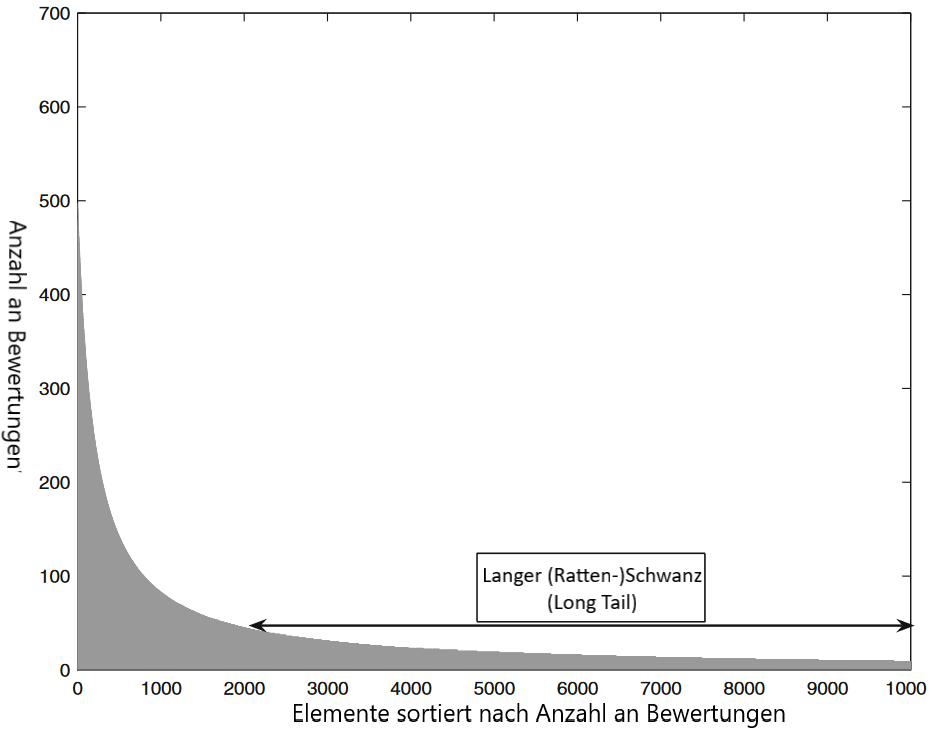
\includegraphics[width=1\textwidth]{gfx/long-tail.png}
	\caption{Darstellung des Long Tails \cite[S. 33]{recommenderSystems:2016}}
	\label{fig:empfehlungssysteme:cf:speicherbasiert:abb1}
\end{figure}

Die in Abbildung \ref{fig:empfehlungssysteme:cf:speicherbasiert:abb1} dargestellte Häufigkeitsverteilung von abgegebenen Bewertungen spiegelt \textcite[S. 1ff.]{anderson:2007} zu Folge einen allgemeinen Trend wider, welchen er im Zusammenhang mit der Digitalisierung beobachtete. Der Autor stellte fest, dass sich Menschen aufgrund der heute verfügbaren breiten Angebote wesentlich diverser orientieren, als es vor einigen Jahrzehnten der Fall war.

Das Sparsity Problem kann auch in Tabelle \ref{tbl:empfehlungssysteme:arbeitsweise:tbl1} beobachtet werden. Dort haben MongoDB und Spark jeweils nur eine Bewertung. Für diese Fähigkeiten ist es über Ähnlichkeitsberechnungen im Bereich des speicherbasierten kollaborativen Filterns somit nicht möglich, für alle Angestellten robuste Vorhersagen zu ermitteln.

Um diesem Problem zu begegnen, kann die bisher verwendete Matrixdarstellung in die Form eines bipartiten Graphen überführt werden \cite[S. 2f.]{huang:2004}. Diese Datenstruktur zeichnet sich durch die Verwendung zwei unterschiedlicher Arten von Knoten zur separaten Speicherung von Nutzern und Elementen aus. Bewertungen werden bei dieser Darstellungsform über gewichtete Kanten im Graphen dargestellt \cite[S. 1f.]{cao:2021}.

Abbildung \ref{fig:empfehlungssysteme:cf:speicherbasiert:abb2} zeigt die Fähigkeitsmatrix aus Tabelle \ref{tbl:empfehlungssysteme:arbeitsweise:tbl1} in der Datenstruktur eines bipartiten Graphen. In der Grafik sind die Knoten der Mitarbeiter rot und die Knoten der Fähigkeiten blau markiert.

\begin{figure}[h]
	\centering	
	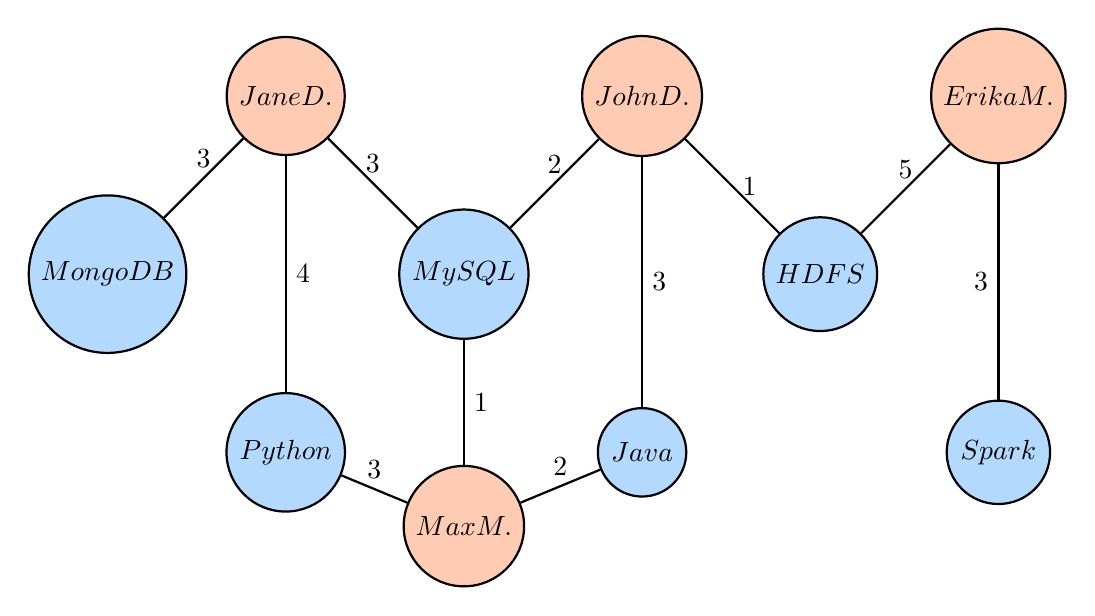
\begin{tikzpicture}[node distance={32mm}, thick, main/.style = {draw, circle}] 
		\node[main, fill=itemcolor] (MongoDB) {$MongoDB$}; 
		\node[main, fill=itemcolor] (Python) [below right of=MongoDB] {$Python$}; 
		\node[main, fill=itemcolor] (MySQL) [above right of=Python] {$MySQL$}; 
		\node[main, fill=itemcolor] (Java) [below right of=MySQL] {$Java$}; 
		\node[main, fill=itemcolor] (HDFS) [above right of=Java] {$HDFS$}; 
		\node[main, fill=itemcolor] (Spark) [below right of=HDFS] {$Spark$};
		
		\node[main, fill=usercolor] (Jane) [above right of=MongoDB] {$Jane D.$}; 
		\node[main, fill=usercolor] (John) [above left of=HDFS] {$John D.$}; 
		\node[main, fill=usercolor] (Max) [below of=MySQL] {$Max M.$};
		\node[main, fill=usercolor] (Erika) [above right of=HDFS] {$Erika M.$}; 
		
		\draw (Jane) -- node[midway, right] {4} (Python);
		\draw (Jane) -- node[midway, above] {3} (MySQL);
		\draw (Jane) -- node[midway, above] {3} (MongoDB);

		\draw (John) -- node[midway, right] {1} (HDFS);		
		\draw (John) -- node[midway, right] {3} (Java);
		\draw (John) -- node[midway, above] {2} (MySQL);
		
		%\path (Erika) edge[bend right=10] node[midway, right] {5} (HDFS); 
		\draw (Erika) -- node[midway, above] {5} (HDFS);
		\draw (Erika) -- node[midway, left] {3} (Spark);
		
		\draw (Max) -- node[midway, above] {2} (Java);
		\draw (Max) -- node[midway, above] {3} (Python);
		\draw (Max) -- node[midway, right] {1} (MySQL);
	\end{tikzpicture}

	\caption{Darstellung der Fähigkeitsmatrix aus Tabelle \ref{tbl:empfehlungssysteme:arbeitsweise:tbl1} in der Datenstruktur eines Graphen}
	\label{fig:empfehlungssysteme:cf:speicherbasiert:abb2}
\end{figure}

\textcite[S. 7ff.]{huang:2004} bemerkten mit Blick auf bipartite Graphen, dass bei klassischen nachbarschaftsbasierten Algorithmen nur Empfehlungen für Knoten bestimmt werden können, welche von einem Zielknoten über drei Kanten zu erreichen sind. Somit könnten in der vorliegenden Abbildung \ref{fig:empfehlungssysteme:cf:speicherbasiert:abb2} über solche Verfahren beispielsweise keine Bewertungsvorhersagen für Jane Doe und Spark oder Erika Muster und MongoDB bestimmt werden.

Um auch in solchen Fällen Empfehlungen zu generieren, ist der Einsatz graphenbasierter Algorithmen empfehlenswert. Diese können über transitive Verbindungen auch weiter entfernte Knoten in die Berechnung mit einbeziehen \cite[S. 60f.]{recommenderSystems:2016}.

Ein in der Literatur häufig angewendeter Graphenalgorithmus ist die Katz-Zentralität \cite[S. 1ff.]{zhan:2017}\cite[S. 6]{guns:2014}\cite[S. 1f.]{huang:2004}. Diese basiert auf einem im Jahr 1953 vorgestellten mathematischen Verfahren von \textcite[S. 1ff.]{katz:1953}. Dieses entwickelte der der Wissenschaftler zur Bestimmung von Anführern in sozialen Gruppen. Heute nutzen graphenbasierte Empfehlungssysteme die Katz-Zentralität unter anderem zur Verbindungsvorhersage (Link Prediction). Diese Problemstellung ist beispielsweise im Bereich der sozialen Netzwerke verbreitet. Sie verfolgt das Ziel, aus vorhandenen Kanten im Graphen bisher unbekannte Verbindungen vorherzusagen \cite[S. 1ff.]{libenNowell:2007}.

Nah verwandt mit der Katz-Zentralität ist Googles PageRank-Algorithmus \cite[S. 1]{was:2018}. Dieser nutzt Kanten zur Darstellung von Verlinkungen im Internet. Auf dieser Grundlage bestimmte Google in seiner Anfangszeit die Wichtigkeit von Webseiten, welche in den Ergebnissen der Suchmaschine entsprechend priorisiert ausgegeben wurden \cite[S. 3ff.]{page:1999}.

Die Katz-Zentralität kann über folgende Gleichung \ref{frml:empfehlungssysteme:cf:speicherbasiert:formel4} bestimmt werden \cite[S. 4]{libenNowell:2007}:
\begin{equation}
	(I - \beta * M)^{-1} - I
	\label{frml:empfehlungssysteme:cf:speicherbasiert:formel4}
\end{equation}
In Gleichung \ref{frml:empfehlungssysteme:cf:speicherbasiert:formel4} steht $\beta$ für eine Zahl im Bereich von null bis eins \cite[S. 6]{guns:2014}, welche jedoch stets kleiner als $\frac{1}{\lambda}$ sein muss. $\lambda$ entspricht dabei dem größten Eigenwert der Matrix M \cite[S. 6]{zhan:2017}. Je größer der Wert von $\beta$ angesetzt wird, desto stärker werden weit entfernte Beziehungen in der Berechnung gewichtet \cite[S. 6]{guns:2014}.

Die Variable $M$ steht in Gleichung \ref{frml:empfehlungssysteme:cf:speicherbasiert:formel4} für die Adjazenzmatrix des betrachteten Graphen \cite[S. 4]{libenNowell:2007}. Diese gibt an, wie viele Kanten von einem Startknoten (Zeile) zu jedem anderen Knoten (Spalte) führen \cite[S. 6]{guns:2014}.

Der mit Zahlen versehene Bereich von Tabelle \ref{tbl:empfehlungssysteme:arbeitsweise:tbl2} entspricht der Adjazenzmatrix für den Graphen aus Abbildung \ref{fig:empfehlungssysteme:cf:speicherbasiert:abb2}.

\begin{table}[h]
	\centering
	\begin{tabular}{c|c|c|c|c|c|c|c|c|c|c}
		& \begin{sideways}Jane D.\end{sideways} & \begin{sideways}John D.\end{sideways} & \begin{sideways}Erika M.\end{sideways} & \begin{sideways}Max M.\end{sideways} & \begin{sideways}Java\end{sideways} & \begin{sideways}Python\end{sideways} & \begin{sideways}MySQL\end{sideways} & \begin{sideways}MongoDB\end{sideways} & \begin{sideways}HDFS\end{sideways} & \begin{sideways}Spark\end{sideways} \\
		\hline
		Jane D.  & 0 & 0 & 0 & 0 & 0 & 4 & 3 & 3 & 0 & 0\\
		John D.  & 0 & 0 & 0 & 0 & 3 & 0 & 2 & 0 & 1 & 0\\
		Erika M. & 0 & 0 & 0 & 0 & 0 & 0 & 0 & 0 & 5 & 3\\
		Max M.   & 0 & 0 & 0 & 0 & 2 & 3 & 1 & 0 & 0 & 0\\
		Java     & 0 & 3 & 0 & 2 & 0 & 0 & 0 & 0 & 0 & 0\\
		Python   & 4 & 0 & 0 & 3 & 0 & 0 & 0 & 0 & 0 & 0\\
		MySQL    & 3 & 2 & 0 & 1 & 0 & 0 & 0 & 0 & 0 & 0\\
		MongoDB  & 3 & 0 & 0 & 0 & 0 & 0 & 0 & 0 & 0 & 0\\
		HDFS     & 0 & 1 & 5 & 0 & 0 & 0 & 0 & 0 & 0 & 0\\
		Spark    & 0 & 0 & 3 & 0 & 0 & 0 & 0 & 0 & 0 & 0
	\end{tabular}
	\caption{Anzahl an Verbindungen im Graphen aus Abbildung \ref{fig:empfehlungssysteme:cf:speicherbasiert:abb2}}
	\label{tbl:empfehlungssysteme:arbeitsweise:tbl2}
\end{table}

%Der mit Zahlen versehene Bereich von Tabelle \ref{tbl:empfehlungssysteme:arbeitsweise:tbl2} entspricht der Adjazenzmatrix des Graphen aus Abbildung \ref{fig:empfehlungssysteme:cf:speicherbasiert:abb2}.

Für Tabelle \ref{tbl:empfehlungssysteme:arbeitsweise:tbl2} ergeben sich mit $\beta = 0.125$ durch Bestimmung der Katz-Zentralität die in Tabelle \ref{tbl:empfehlungssysteme:arbeitsweise:tbl3} dargestellten Werte. Die vollständige Berechnung kann in Appendix \ref{ch:nebenrechnungen:katzZentralitaet} nachvollzogen werden.
\newpage
\begin{table}[h]
	\centering
	\begin{tabular}{c|c|c|c|c|c|c|c|c|c|c}
		& \begin{sideways}Jane D.\end{sideways} & \begin{sideways}John D.\end{sideways} & \begin{sideways}Erika M.\end{sideways} & \begin{sideways}Max M.\end{sideways} & \begin{sideways}Java\end{sideways} & \begin{sideways}Python\end{sideways} & \begin{sideways}MySQL\end{sideways} & \begin{sideways}MongoDB\end{sideways} & \begin{sideways}HDFS\end{sideways} & \begin{sideways}Spark\end{sideways} \\ 
		\hline
		Jane D.  & 1.66 & 0.47 & 0.08 & 0.87 & 0.39 & 1.66 & 1.22 & 1.00 & 0.11 & 0.03\\
		John D.  & 0.47 & 0.42 & 0.24 & 0.37 & 0.62 & 0.37 & 0.58 & 0.18 & 0.33 & 0.09\\
		Erika M. & 0.08 & 0.24 & 1.17 & 0.06 & 0.10 & 0.06 & 0.10 & 0.03 & 1.39 & 0.81\\
		Max M.   & 0.87 & 0.37 & 0.06 & 0.60 & 0.54 & 1.04 & 0.62 & 0.33 & 0.08 & 0.02\\
		Java     & 0.39 & 0.62 & 0.10 & 0.54 & 0.37 & 0.40 & 0.37 & 0.15 & 0.14 & 0.04\\
		Python   & 1.66 & 0.37 & 0.06 & 1.04 & 0.40 & 1.22 & 0.84 & 0.62 & 0.09 & 0.02\\
		MySQL    & 1.22 & 0.58 & 0.10 & 0.62 & 0.37 & 0.84 & 0.68 & 0.46 & 0.13 & 0.04\\
		MongoDB  & 1.00 & 0.18 & 0.03 & 0.33 & 0.15 & 0.62 & 0.46 & 0.37 & 0.04 & 0.01\\
		HDFS     & 0.11 & 0.33 & 1.39 & 0.08 & 0.14 & 0.09 & 0.13 & 0.04 & 0.91 & 0.52\\
		Spark    & 0.03 & 0.09 & 0.81 & 0.02 & 0.04 & 0.02 & 0.04 & 0.01 & 0.52 & 0.31
	\end{tabular}
	\caption{Berechnete Katz-Zentralität mit $\beta = 0.125$ für Tabelle \ref{tbl:empfehlungssysteme:arbeitsweise:tbl2}}
	\label{tbl:empfehlungssysteme:arbeitsweise:tbl3}
\end{table}

In Tabelle \ref{tbl:empfehlungssysteme:arbeitsweise:tbl3} ist zu erkennen, dass durch Bestimmung der Katz-Zentralität für sämtliche Knoten die Stärke der Verbindung zu allen anderen Knoten vorhergesagt werden konnte. Das Sparsity Problem wurde somit behoben. Die vorliegenden Ergebnisse eigenen sich folglich sehr gut, um auf deren Basis Ähnlichkeiten zwischen Nutzern oder Fähigkeiten zu bestimmen.

Allerdings ist auch festzustellen, dass die Skalierung der Bewertungen verändert wurde. Projekt-Anforderungen, welche auf der in Tabelle \ref{tbl:empfehlungssysteme:arbeitsweise:tbl2} verwendeten Bewertungsskala spezifiziert wurden, könnte ein Algorithmus somit nicht ohne weiteres mit den Ergebnissen aus Tabelle \ref{tbl:empfehlungssysteme:arbeitsweise:tbl3} abgleichen.

Eine Lösungsmöglichkeit zeigen Algorithmen von Gruppen-Recommender Engines auf. Solche Systeme verfolgen das Ziel, gemeinsame Vorschläge für mehrere Anwender zu generieren \cite[S. 1]{dara:2020}. Ein in diesem Zusammenhang angewendetes Verfahren ist das Erstellen eines Pseudonutzers, welcher die Präferenzen aller Gruppenmitglieder vereint. Der Pseudonutzer wird bei Empfehlungsberechnung als gewöhnlicher Anwender betrachtet und beispielsweise in Tabelle \ref{tbl:empfehlungssysteme:arbeitsweise:tbl1} in eine neue Zeile eingefügt. Dieses Vorgehen ermöglicht es, die bisher vorgestellten Verfahren im Bereich des kollaborativen Filterns ohne zusätzlich Komplexität auch zur Bestimmung von Vorschlägen für Gruppen anzuwenden \cite[S. 8f.]{oconnor:2001}.

Ein vergleichbarer Ansatz könnte auch zur Bestimmung der Katz-Zentralität genutzt werden. Hierfür müsste ein Algorithmus zunächst Tabelle \ref{tbl:empfehlungssysteme:arbeitsweise:tbl2} um eine Zeile erweitern, in welcher das zu besetzende Projekt mitsamt den dafür benötigten Fähigkeiten als Pseudomitarbeiter einfügt wird. Nach der anschließenden Bestimmung der Katz-Zentralität würden auch die Fähigkeiten des Pseudomitarbeiters der neuen Skalierung entsprechen. Somit könnten diese neuen Fähigkeitsbewertungen als Ausgangspunkt für die Bestimmung passender Mitarbeiter für das Projekt verwendet werden. Ein vergleichbares Verfahren wendeten auch \textcite[S. 2]{mitre:2014} bei der Implementierung ihres Empfehlungssystems zur Projektbesetzung an. Die Wissenschaftler nutzen jedoch klassische Verfahren zur Ähnlichkeitsberechnung und keine Graphenalgorithmen.

Unabhängig von der konkreten Art der Implementierung ist ein großer Nachteil an speicherbasierten Verfahren, dass bei jeder Empfehlungsberechnung sämtliche Nutzer, Elemente und Bewertungen in den Hauptspeicher geladen werden müssen \cite[S. 8]{yang:2016}. Zusätzlich ist festzustellen, dass häufig sehr hohe Laufzeiten zu erwarten sind \cite[S. 2]{zhang:2010}. So bemerken beispielsweise \textcite[S. 3]{landherr:2010}, dass alleine die Matrix-Invertierung zur Bestimmung der Katz-Zentralität mit Gleichung \ref{frml:empfehlungssysteme:cf:speicherbasiert:formel4} eine Komplexität von $O(n^3)$ besitzt. Aus diesen Gründen ist die Verwendung speicherbasierter Ansätze bei großen Datensätzen als ungeeignet zu bewertet. Abhilfe bei steigender Datenmenge können modellbasierte Verfahren bieten \cite[S. 8]{yang:2016}.


\subsection{Modellbasierte Verfahren}
\label{ch:empfehlungssysteme:cf:modellbasiert}
Modellbasierte Verfahren verwenden Ansätze aus dem Bereich des Data Minings zur Generierung von Vorschlägen. Hierbei berechnen Wissenschaftler statistische Modelle, bevor sie ihr Empfehlungssystem den Nutzern zur Verfügung stellen \cite[S. 2]{cui:2020}. Dieses Vorgehen hat den Vorteil, dass in der Produktivumgebung keine Berechnungen mehr auf allen Daten ausgeführt werden müssen. Somit ist die Vorschlagsbestimmung insbesondere bei großen Datenmengen effizienter als bei speicherbasierten Verfahren \cite[S. 8]{yang:2016}.

Wie in Tabelle \ref{tbl:empfehlungssysteme:cf:modellbasiert:tbl1} dargestellt, ist es bei modellbasierten Verfahren üblich, den vorhandenen Datensatz in Trainings- (rot) und Testdaten (blau) zu untergliedern \cite[S. 71f.]{recommenderSystems:2016}. Die Einteilung in der Tabelle erfolgte zufällig.%Bei Modellentwicklungen zur Vervollständigung von Matrizen nutzen Wissenschaftler häufig die beobachteten Felder als Trainings- und die unbeobachteten Einträge als Testdaten \cite[S. 71f.]{recommenderSystems:2016}. Die Aufteilung kann beispielsweise im Verhältnis von 80 Prozent Trainings- und 20 Prozent Testdaten erfolgen \cite[S. 12]{najafabadi:2017}. 

\begin{table}[h]
	\centering
	\begin{tabular}{c|c|c|c|c|c|c}
		& Java & Python & MySQL & MongoDB & HDFS & Spark\\ 
		\hline
		Doe, Jane 		& \cellcolor{itemcolor}2 & \cellcolor{usercolor}4 & \cellcolor{itemcolor}3 & \cellcolor{usercolor}3 & \cellcolor{itemcolor}2 & \cellcolor{usercolor}1\\
		Doe, John 		& \cellcolor{usercolor}3 & \cellcolor{itemcolor}4 & \cellcolor{usercolor}2 & \cellcolor{usercolor}1 & \cellcolor{usercolor}1 & \cellcolor{itemcolor}3\\
		Muster, Erika 	& \cellcolor{itemcolor}5 & \cellcolor{itemcolor}2 & \cellcolor{itemcolor}3 & \cellcolor{usercolor}2 & \cellcolor{usercolor}5 & \cellcolor{usercolor}3\\
		Muster, Max 	& \cellcolor{usercolor}2 & \cellcolor{usercolor}3 & \cellcolor{usercolor}1 & \cellcolor{itemcolor}4 & \cellcolor{usercolor}1 & \cellcolor{itemcolor}2
	\end{tabular}
	\caption{Beispiel für eine Matrixdarstellung von Fähigkeiten mit Unterteilung in Trainings- und Testdaten}
	\label{tbl:empfehlungssysteme:cf:modellbasiert:tbl1}
\end{table}

Die Trainingsdaten werden genutzt, um statistische Modelle zur Vorhersage von Bewertungen zu entwickeln \cite[S. 71f.]{recommenderSystems:2016}. Die Testdaten dienen zur anschließenden Evaluierung und Bewertung hinsichtlich der Genauigkeit des erstellten Modells. Hierbei ist es beispielsweise möglich, bekannte Einträge von Testdaten in der Matrix temporär zu entfernen, diese anschließend durch das trainierte Modell vorherzusagen und daraufhin tatsächliche und vorhergesagte Werte zu vergleichen \cite[S. 3ff.]{kang:2016}.
% die Implementierung neuronaler Netze \cite[S. 5ff.]{personJobFit:2018}, die Anwendung des naiven Bayes-Klassifikators \cite[S. 2]{valdividezodiaz:2019}, die Durchführung von Matrix-Faktorisierungsverfahren \cite[S. 2ff.]{ortega:2016} oder die Berechnung von Entscheidungsbäumen \cite[S. 1ff.]{yu:2012} verbreitet.

Wie an den Spalten in Tabelle \ref{tbl:empfehlungssysteme:cf:modellbasiert:tbl1} zu erkennen ist, existieren in der Praxis häufig sehr viele Merkmale bzw. Dimensionen, welche zur Entwicklung von Modellen relevant sein können. Zusätzlich sind Matrizen, wie in Kapitel \ref{ch:empfehlungssysteme:cf:speicherbasiert} beschrieben, in der Praxis aufgrund des Sparsity Problems meist sehr schwach besetzt. \textcite[S. 1]{boratto:2014} stellten fest, dass in solchen Situationen, in welchen viele Dimensionen und gleichzeitig wenigen Daten vorliegen, keine statistisch aussagekräftigen Modelle erstellt werden können. \textcite[S. 94]{bellman:1961} prägte für diesen Sachverhalt den Ausdruck "Fluch der Dimensionalität"\footnote{"Curse of dimensionality" - \textcite[S. 94]{bellman:1961}}. Um in solchen Situationen dennoch Empfehlungen generieren zu können, stellten verschiedene Autoren in der Literatur Verfahren zur Dimensionsreduzierung vor. Verbreitet ist dabei beispielsweise die Hauptkomponentenanalyse, welche im englischsprachigen Raum als \ac{PCA} bezeichnet wird \cite[S. 1ff.]{vaswani:2018}.

\textcite[S. 1f.]{pennock:2000} kritisierten an modellbasierten Verfahren, dass diese stets den Zustand der Daten zum Zeitpunkt des Trainings des Modells abbilden. Werden beispielsweise Fähigkeiten in der Datenbank hinzugefügt bzw. entfernt oder Bewertungen signifikant verändert, muss gegebenenfalls das statistische Modell neu trainiert werden, um diese Anpassungen zu erfassen. Speicherbasierte Verfahren können den Autoren zu Folge solche Änderungen dagegen unmittelbar berücksichtigen.

Ein Problem, welches weder speicher- noch modellbasierte Verfahren im Bereich des kollaborativen Filterns zuverlässig lösen können, ist der sogenannte Kaltstart (Cold Start). Dieser tritt auf, wenn neue Nutzer oder Fähigkeiten in die Datenbank hinzugefügt werden, welchen noch keine Bewertung zugeordnet ist \cite[S. 5]{huang:2004}. In solchen Fällen ist die gesamte Zeile bzw. Spalte in Tabelle \ref{tbl:empfehlungssysteme:arbeitsweise:tbl1} mit fehlenden Einträgen gekennzeichnet. Im entsprechenden Graphen in Abbildung \ref{fig:empfehlungssysteme:cf:speicherbasiert:abb2} existiert somit keine Kante von der betrachteten Entität zu anderen Knoten. Daher ist es weder über speicherbasierte Ähnlichkeitsberechnungen, noch graphenbasierte Algorithmen oder statistische Modelle möglich, zuverlässige Vorhersagen mittels kollaborativem Filtern zu bestimmen. Eine Lösung für den Kaltstart können Verfahren im Bereich des inhaltsbasierten Filterns bieten. % Quelle

\section{Inhaltsbasiertes Filtern}
\label{ch:empfehlungssysteme:inhaltsbasiertesFiltern}
Verfahren des inhaltsbasierten Filterns nutzen im Unterschied zum kollaborativen Filtern keine Daten anderer Anwender zur Bestimmung von Vorhersagen. Algorithmen in diesem Bereich fokussieren Beschreibungen von Nutzern und Elementen \cite[S. 139f.]{recommenderSystems:2016}.

Soll analog zum Beispiel aus Kapitel \ref{ch:empfehlungssysteme:cf:speicherbasiert} die Javabewertung von Jane Doe vorhergesagt werden, würden beim inhaltsbasierten Filtern somit keine Ähnlichkeitsberechnungen zwischen Java und jeder anderen Fähigkeit bzw. Jane Doe und allen anderen Mitarbeitern durchgeführt werden. Stattdessen könnten beispielsweise Satzbausteine im Lebenslauf von Jane Doe mit Wörtern in entsprechender Fachliteratur zu Javatechnologien verglichen werden.

Solche Anwendungen im Bereich des inhaltsbasierten Filterns implementierten beispielsweise \textcite[S. 4ff.]{guo:2016} und \textcite[S. 3ff.]{prospect:2010}. Diese entwickelten Empfehlungssysteme zur Stellensuche bzw. -besetzung. In beiden Fällen nutzten die Wissenschaftler Methoden aus der Computerlinguistik, um aus unstrukturierten Stellenausschreibungen und Lebensläufen semantische Merkmale zu extrahieren. Die dabei gewonnenen Daten speicherten sie einer strukturierten Form, welche den Forschern die Anwendung von Ähnlichkeitsberechnungen ermöglichte. Über diese bestimmten \textcite[S. 4ff.]{guo:2016} die Übereinstimmungen im Lebenslauf eines Anwenders mit vorhandenen Stellenbeschreibungen in deren Datenbank. Die als am relevantesten bewerteten Gesuche wurden an den Nutzer zurückgegeben. Ähnlich arbeitete auch das Empfehlungssystem von \textcite[S. 3ff.]{prospect:2010}. Diese bestimmten die Ähnlichkeit zwischen den Lebensläufen von Bewerbern und einer zu besetzenden Stelle, um Personalsachbearbeiter bei der Kandidatenauswahl zu unterstützen.

% Das doppelt sich
Auch \textcite[S. 1ff.]{almalis:2014} entwickelten ein inhaltsbasiertes Empfehlungssystem, welches geeignetes Personal für offene Stellen bestimmte. Hierbei überführten Sie unstrukturierte Stellenanforderungen und Lebensläufe der Kandidaten in die Form einheitlicher Vektoren. Über Ähnlichkeitsberechnungen bestimmten die Wissenschaftler diejenigen Personen, welche die höchste Übereinstimmung mit den gesuchten Anforderungen aufweisen konnten.

Auch ist es möglich, graphenbasierte Verfahren im Bereich des inhaltsbasierten Filterns  einzusetzen. Diese bieten die Möglichkeit, vorhandene Daten über Ontologien miteinander zu verbinden. So entwickelten beispielsweise \textcite[S. 1ff.]{kumaran:2013} ein IT-System, welches Bewerbungen und Stellenausschreibungen über Verfahren der Computerlinguistik in einheitliche Ontologien überträgt. Auch hier ermittelten die Wissenschaftler über Ähnlichkeitsberechnungen die geeignetsten Bewerber für offene Stellen.

Es wäre ebenso denkbar, die von \textcite[S. 1ff.]{kumaran:2013} entwickelten Ontologien um weiteres Domänenwissen anzureichern und dieses in den Vorschlagsprozess einzubeziehen. Ein solches Vorgehen verfolgen wissensbasierte Empfehlungssysteme \cite[S. 168f.]{recommenderSystems:2016}.% Da auch diese Anwendungen Vorschläge auf Basis der Eigenschaften von Nutzern und Elementen generieren, wird in der Literatur diskutiert, ob es sich bei wissens- und inhaltsbasierten Empfehlungssystemen um separate Gattungen von Recommender Engines handelt.

\section{Wissensbasierte Empfehlungssysteme}
\label{ch:empfehlungssysteme:wissensbasierteAnsaetze}
% Anmerkung Andreas (21. Juni): Esco ist sehr allgemein
Beim Erstellen von wissensbasierten Empfehlungssystemen können Unternehmen auf bereits vorhandene Ontologien zurückgreifen. Beispielsweise stellt die Europäische Kommission mit \acs{ESCO} (\acl{ESCO}) explizit zum Zweck der Stellenbesetzung eine mehrsprachige Ontologie mit vordefinierten Kompetenzen, Fähigkeiten und Qualifikationen bereit \cite[S. 1ff.]{leVrang:2014}. Ein vergleichbares Angebot existiert mit \acs{ONet} (\acl{ONet}) auch von der Regierung der Vereinigten Staaten von Amerika \cite[S. 2]{aCombinedRepresentation:2018}.

In solchen Wissensdatenbanken können Unternehmen zu Stellen passende Mitarbeiter über semantische Suchen abfragen. Hierbei kann das System über hinterlegte Regeln sowohl Synonyme als auch Beziehungen berücksichtigen \cite[S. 2f.]{singto:2013}. Jedoch werden dabei Mitarbeiter in den Ergebnissen nur ausgegeben, wenn sie die Suchanfrage exakt erfüllen. Aus diesem Grund stellten \textcite[S. 3]{bianchini:2008} bei semantischen Suchen eine hohe Genauigkeit der Resultate fest, bemängelten jedoch die Flexibilität der Verfahren.

Auch ist es möglich, innerhalb der Ontologien über Graphenalgorithmen die Übereinstimmungen zwischen Fähigkeiten zu berechnen \cite[S. 1f.]{balachander:2018}. Bei solchen, auf Ähnlichkeitsberechnungen basierenden Verfahren, beobachteten \textcite[S. 4]{bianchini:2008} eine hohe Flexibilität, kritisierten jedoch die mangelnde Genauigkeit der Verfahren.

Um die Nachteile beider Ansätze auszugleichen, implementierten \textcite[S. 4ff.]{semanticMatchmaking:2009} ein eigenes Empfehlungssystem. Dieses sollte gleichzeitig eine hohe Genauigkeit und Flexibilität gewährleisten. Für dieses Vorhaben entwickelten die Wissenschaftler eine Ontologie, welche die Fähigkeiten der Mitarbeiter sehr feingranular erfasste. Einzelne Kompetenzen mussten dabei über mehrere Einträge spezifiziert werden. Zu Stellen passende Personen wurden anschließend über einen Algorithmus ermittelt, welcher semantische Schlussfolgerungen mit Ähnlichkeitsberechnungen kombinierte. Mit diesem Ansatz erreichten \textcite[S. 11f.]{semanticMatchmaking:2009} ihr Ziel, ein genaues und zugleich flexibles wissensbasiertes Empfehlungssystem zu implementieren. Jedoch muss kritisch angemerkt werden, dass die Pflege der Fähigkeiten in der Ontologie als sehr aufwändig erscheint. Somit muss in Frage gestellt werden, ob Mitarbeiter ein solches System zuverlässig im Unternehmensalltag pflegen würden. Auch \textcite[S. 2]{aCombinedRepresentation:2018} beobachten in anderen Job-Ontologien wie \acs{ONet}, dass Informationen über Fähigkeiten häufig nicht aktuell gehalten werden.

Die von \textcite[S. 1]{semanticMatchmaking:2009} implementierte Recommener Engine kombinierte semantische Schlussfolgerungen und Ähnlichkeitsberechnungen in einem System. Aus diesem Grund kann deren Anwendung auch als hybrides Empfehlungssystem bezeichnet werden.

\section{Hybride Empfehlungssysteme}
\label{ch:empfehlungssysteme:hybrideEmpfehlungssysteme}
Hybride Systeme verwenden innerhalb einer Anwendung mehrere unterschiedliche Empfehlungsansätze. Dadurch können sie die Nachteile einzelner Verfahren ausgleichen bzw. die Vorteile mehrerer Ansätze miteinander verbinden, um die Qualität der Ergebnisse zu verbessern \cite[S. 199f.]{recommenderSystems:2016}\cite[S. 8]{malinowski:2008}.

Beispielsweise entwickelten \textcite[S. 1ff.]{shalaby:2017} ein hybrides Empfehlungssystem für eine Website zur Stellensuche. Dabei bezogen sie mehrere Datenquellen in den Vorschlagsprozess ein und kombinierten dabei unter anderem graphen- und modellbasierte Methoden. Ihr hybrides System verglichen die Wissenschaftler in einem A/B-Test mit dem auf der Website bisher eingesetzten modellbasierten Verfahren aus dem Bereich des kollaborativen Filterns. Hierbei konnten sie nachweisen, dass die Nutzer höheres Interesse an den Stellen des hybriden Empfehlungssystems aufzeigten. Jedoch muss die Evaluation kritisch betrachtet werden. \textcite[S. 10f.]{stegemann:2020} empfahlen, bei A/B-Tests bei jeder zu testenden Variante jeweils nur ein Merkmal zu verändern. Ansonsten kann den Autoren zu Folge in der Evaluation nicht mit Sicherheit bestimmt werden, welche Anpassung zur Veränderung des Nutzerverhaltens führte. \textcite[S. 1ff.]{shalaby:2017} änderten in ihrem System jedoch mehrere Merkmale in der neuen Variante. So nutzten sie unter anderem anstelle des kollaborativen Filterns hybride Verfahren und verwendeten zusätzlich mehr Datenquellen als die vorherige Variante. Somit kann nicht mit Sicherheit festgestellt werden, dass die verbesserten Ergebnisse auf den Einsatz des hybriden Systems zurückzuführen ist. Auch wäre es denkbar, dass die Einbeziehung der zusätzlichen Datenquellen zum veränderten Nutzerverhalten führte.

Zu aussagekräftigeren Ergebnissen kamen \textcite[S. 1ff.]{combiningCbAndCFCostSensitiveApproach:2017}. Die Wissenschaftler implementierten ein hybrides, modellbasiertes Empfehlungssystem zur Stellensuche. Dabei kombinierten sie kollaboratives und inhaltsbasiertes Filtern. Zur Evaluation teilten die Forscher ihren vorhandenen Datensatz in Trainings- und Testdaten. Anschließend verglichen sie die Präzision des rein inhaltsbasierten Ansatzes mit der Kombination aus inhaltsbasiertem Ansatz und kollaborativem Filtern. Hierbei stellten fest, dass der hybride Ansatz zu besseren Ergebnissen führte.

Auch für die Personalauswahl wurden in der Literatur hybride Empfehlungssysteme entwickelt. Beispielsweise implementierten \textcite[S. 1ff.]{mohamed:2018} eine Anwendung bestehend aus wissens- und inhaltsbasierten Verfahren. Dieses sortierte vorhandene Lebensläufe entsprechend den Anforderungen von Personalsachbearbeiten. Zu diesem Zweck überführten die Wissenschaftler die Lebensläufe der Kandidaten zunächst über Methoden der Computerlinguistik in einheitliche Ontologien. Personalsachbearbeiter konnten über eine Suchmaske Anforderungen spezifizieren. Über Ähnlichkeitsberechnungen zwischen Lebensläufen und Schlüsselworten bestimmten die Wissenschaftler für jeden Kandidaten eine Profilbewertung zur Sortierung. Dabei nutzten die Forscher für gesuchte und vorhandene Fähigkeiten eine einheitliche Ontologie, über welche sie Ähnlichkeiten bestimmten. Zur Evaluation des Systems ließen die Wissenschaftler vorhandene Lebensläufe entsprechend vorgegebener Stellenspezifikationen sowohl von ihrem System als auch von erfahrenen Personalsachbearbeitern sortieren. Hierbei stellten sie fest, dass die Ergebnisse ihrer Anwendung vergleichbar mit denen der HR-Angestellten waren. Aus diesen Resultaten wird geschlossen, dass das hybride Empfehlungssystem ähnlich gute Vorschläge in deutlich geringerer Zeit erzielen kann.

%\textcite[S. 16]{hybridImmunizing:2017} zeigten, dass deren hybrides Job-Empfehlungssystem trotz der Kombination mehrerer Verfahren eine nach wie vor sehr hohe Performance aufweisen konnte.
Trotz dieser Ergebnisse kritisierten \textcite[S. 1]{malinowski:2008}, dass ein hybrides Empfehlungssystem nicht ausreicht, um geeignete Mitarbeiter für Stellen zu empfehlen. Deren Einschätzung zu Folge ist die Entwicklung bilateraler Empfehlungssysteme notwendig.
\shorthandon{"}